\documentclass[11pt]{article}

% ---------------------------------------------------------------------------
% template2: a typographic treatment of the same report.
%
% Latin Modern throughout, so text and the 78 inline maths expressions match.
% (Times and Palatino were tried first; this TeX Live install has no Helvetica
% or Palatino metrics, and mathptmx breaks on \Sigma^{-1}.)  The modern feel
% comes from the layout, one navy accent, and restyled figures rather than
% from an exotic typeface.
%
% Figures are read from figs_modern/, produced by make_modern_figs.py in a
% matching Computer Modern style, so report.tex and figs/ are untouched.
% ---------------------------------------------------------------------------

\usepackage[margin=1in]{geometry}
\usepackage{amsmath, amssymb}
\usepackage[T1]{fontenc}
\usepackage{lmodern}
\usepackage{microtype}
\usepackage{graphicx}
\usepackage{booktabs}
\usepackage{array}
\usepackage{float}
\usepackage{xcolor}
\usepackage{fancyhdr}
\usepackage[font=small,labelfont=bf,skip=5pt]{caption}

\definecolor{psink}{RGB}{23,54,93}
\definecolor{psaccent}{RGB}{192,80,77}
\definecolor{psrule}{RGB}{200,209,222}

\usepackage[colorlinks=true,allcolors=psink]{hyperref}

\graphicspath{{figs_modern/}}
\emergencystretch=3em

% spacing: padding around floats is the single biggest lever on length
\setlength{\textfloatsep}{10pt plus 2pt minus 2pt}
\setlength{\intextsep}{10pt plus 2pt minus 2pt}
\setlength{\abovecaptionskip}{4pt}
\setlength{\belowcaptionskip}{0pt}

% headings: navy, small caps for sections, bold below that
% (titlesec is not installed, so the sectioning commands are redefined here)
\makeatletter
\renewcommand\section{\@startsection{section}{1}{0pt}%
  {-2.6ex \@plus -1ex \@minus -.2ex}{1.3ex \@plus .2ex}%
  {\normalfont\scshape\large\color{psink}}}   % lmr has no bold small caps
\renewcommand\subsection{\@startsection{subsection}{2}{0pt}%
  {-2.2ex \@plus -1ex \@minus -.2ex}{1.0ex \@plus .2ex}%
  {\normalfont\bfseries\normalsize\color{psink}}}
\renewcommand\paragraph{\@startsection{paragraph}{4}{0pt}%
  {1.7ex \@plus 1ex \@minus .2ex}{-0.9em}%
  {\normalfont\bfseries\normalsize\color{psink}}}
\makeatother

\pagestyle{fancy}
\fancyhf{}
\fancyhead[L]{\footnotesize\scshape\color{psink} MGT 595 \textemdash\ Problem Set 2}
\fancyhead[R]{\footnotesize\color{psink}\thepage}
\renewcommand{\headrulewidth}{0.4pt}
\renewcommand{\headrule}{\hbox to\headwidth{%
  \color{psrule}\leaders\hrule height \headrulewidth\hfill}}

\newcommand{\todo}[1]{\textcolor{psaccent}{\textbf{[TO WRITE: #1]}}}

\begin{document}

\thispagestyle{empty}
\begin{flushleft}
{\bfseries\LARGE\color{psink} Quantitative Investing}\\[3pt]
{\scshape\Large\color{psink} Problem Set 2}\\[10pt]
{\color{psrule}\rule{\textwidth}{1.2pt}}\\[5pt]
{\small Ashley Wen\,(xw564)\quad\textbar\quad Emily Wu\,(esw63)%
\quad\textbar\quad Grace Gu\,(xg325)\hfill \today}
\end{flushleft}

\vspace{1.4em}

% =====================================================================
\section{Question 1: Mean--Variance Portfolios --- 10 Industries}
% =====================================================================

\paragraph{Data and conventions.} The data are monthly value-weighted returns
on ten U.S.\ industry portfolios from July 1926 to June 2026, giving
$T = 1200$ observations on $N = 10$ industries, with no missing values. All
figures are in percent per month unless stated otherwise: a mean of $1.0584$
means $1.0584\%$ per month. The risk-free rate is the sample mean of the
monthly risk-free column, $r_f = 0.2701\%$ per month. Short sales are
unrestricted, so writing $\mu$ for the vector of sample means, $\Sigma$ for
the sample covariance matrix and $\mathbf{1}$ for a vector of ones,
\begin{equation}
w_{\text{MVP}} = \frac{\Sigma^{-1}\mathbf{1}}{\mathbf{1}'\Sigma^{-1}\mathbf{1}},
\qquad
w_{\text{TAN}} = \frac{\Sigma^{-1}(\mu - r_f\mathbf{1})}
                       {\mathbf{1}'\Sigma^{-1}(\mu - r_f\mathbf{1})},
\label{eq:weights}
\end{equation}
with $\mu_p = w'\mu$, $\sigma_p = \sqrt{w'\Sigma w}$ and
$S_p = (\mu_p - r_f)/\sigma_p$.

\subsection{Question 1(a): MVP, Tangency Portfolio and the Efficient Frontier}

\begin{table}[H]
\centering
\caption{Industry sample moments and the resulting portfolio weights from
equation~\eqref{eq:weights}. Weights sum to one in each column. The last three
rows report the mean, standard deviation, Sharpe ratio, gross leverage and
cross-sectional weight dispersion of each portfolio.}
\small
\begin{tabular}{lrrrr}
\toprule
 & \multicolumn{2}{c}{Monthly (\%)} & \multicolumn{2}{c}{Weight} \\
\cmidrule(lr){2-3}\cmidrule(lr){4-5}
Industry & Mean & Std.\ Dev. & MVP & Tangency \\
\midrule
NoDur & 0.9402 & 4.5595 & 0.7188 & 0.6645 \\
Durbl & 1.1822 & 8.2136 & $-0.0142$ & 0.1340 \\
Manuf & 1.0385 & 6.2008 & $-0.1905$ & $-0.2242$ \\
Enrgy & 1.0292 & 6.4095 & 0.1527 & 0.2808 \\
HiTec & 1.1699 & 7.1424 & $-0.0621$ & 0.1865 \\
Telcm & 0.8124 & 4.6606 & 0.4889 & 0.1525 \\
Shops & 1.0342 & 5.7802 & $-0.0137$ & 0.0725 \\
Hlth & 1.0680 & 5.5005 & 0.1174 & 0.3530 \\
Utils & 0.8874 & 5.4351 & 0.1293 & 0.0721 \\
Other & 0.9237 & 6.3555 & $-0.3267$ & $-0.6916$ \\
\midrule
\textit{Portfolio mean} (\%/mo) &  &  & 0.8672 & 1.0584 \\
\textit{Portfolio std.\ dev.} (\%/mo) &  &  & 3.8346 & 4.4063 \\
\textit{Sharpe ratio} (monthly) &  &  & 0.1557 & 0.1789 \\
\textit{Gross leverage} $\sum_i |w_i|$ &  &  & 2.21 & 2.83 \\
\textit{Cross-sectional SD of weights} &  &  & 0.3085 & 0.3590 \\
\bottomrule
\end{tabular}
\label{tab:q1a}
\end{table}

\begin{figure}[H]
\centering

\includegraphics[width=0.72\textwidth]{q1a_frontier.png}
\caption{Efficient frontier of the ten industries in mean--standard deviation
space. Red dots are the individual industries, the orange square is the
minimum variance portfolio, the green star is the tangency portfolio, and the
dotted line is the capital allocation line from the risk-free rate. The dashed
grey curve is the inefficient lower branch.}
\label{fig:q1a}
\end{figure}


\paragraph{Discussion of the weights.}
\begin{itemize}
\setlength{\itemsep}{4pt}\setlength{\parskip}{0pt}

\item \textbf{NoDur is the largest long position in both portfolios.} It has
the lowest standard deviation of the ten industries and, once the other nine
are controlled for, the lowest residual volatility, which makes it the most
effective hedging instrument in the set. Both objectives want it.

\item \textbf{The two portfolios disagree most on Telcm.} Telcm has the
second-lowest standard deviation and the lowest mean return in the sample.
Minimizing variance alone makes it valuable, and once expected return enters,
its low volatility no longer pays for the weakest risk premium of the ten.

\item \textbf{The tangency portfolio is the more aggressive of the two,
despite holding more industries long.} It carries higher gross leverage and
more dispersed weights. The difference is where the extremity sits: the MVP
concentrates on the long side and spreads small shorts across five industries,
three of them negligible, while the tangency portfolio funds eight longs out
of a single large short in Other, the lowest-Sharpe industry. The extra
leverage is what it costs to bet on mean differences that are small next to an
average pairwise correlation of 0.696.

\end{itemize}

\paragraph{Shape of the frontier.} We minimize portfolio variance, which is
quadratic in the weights, subject to two linear constraints. The optimal
weights then come out as an affine function of the target mean, so every
frontier portfolio is a fixed combination of two underlying portfolios. This
is the two-fund separation result. Substituting that affine function back into
the quadratic objective gives a quadratic again, so variance is quadratic in
the target mean. The minimum-variance set is therefore a parabola in
mean--variance space, and a hyperbola in the mean--standard deviation space of
Figure~\ref{fig:q1a}. Two things follow.

\begin{itemize}
\setlength{\itemsep}{4pt}\setlength{\parskip}{0pt}

\item \textbf{The curvature is diversification.} If the industries were
perfectly correlated, combining them would reduce no risk and the attainable
set would be a straight line. Correlations below one bend it leftward, and how
far it bends measures how much diversification is available. Here the bend is
modest: the MVP is only about a sixth less volatile than the least volatile
industry, where part (c) shows it would be less than half as volatile if the
industries were uncorrelated.

\item \textbf{Dominance makes only the upper branch efficient.} Because
variance is quadratic in the target mean, every variance above the minimum is
attained by two portfolios, one on each side of the minimum variance
portfolio. They carry identical risk but the lower one returns less, so it is
dominated. Since investors prefer a higher expected return at the same risk,
no one would hold it: the lower branch is feasible but never optimal, which is
why it is dashed in Figure~\ref{fig:q1a}.

\end{itemize}

\subsection{Question 1(b): Reliability of the Mean Return Estimates}

The standard error of each sample mean is $\hat\sigma_i/\sqrt{T}$ with
$T = 1200$.

\begin{table}[H]
\centering
\caption{Reliability of the estimated mean returns, annualized. The
$t$-statistic tests the null that the true mean return is zero.}
\small
\begin{tabular}{lrrr}
\toprule
Industry & Mean (\%/yr) & Std.\ Error (\%/yr) & $t$-statistic \\
\midrule
NoDur & 11.28 & 1.58 & 7.14 \\
Durbl & 14.19 & 2.85 & 4.99 \\
Manuf & 12.46 & 2.15 & 5.80 \\
Enrgy & 12.35 & 2.22 & 5.56 \\
HiTec & 14.04 & 2.47 & 5.67 \\
Telcm & 9.75 & 1.61 & 6.04 \\
Shops & 12.41 & 2.00 & 6.20 \\
Hlth & 12.82 & 1.91 & 6.73 \\
Utils & 10.65 & 1.88 & 5.66 \\
Other & 11.08 & 2.20 & 5.03 \\
\bottomrule
\end{tabular}
\label{tab:q1b_rel}
\end{table}

We then raise every estimated mean by one of its own standard errors,
$\tilde\mu_i = \hat\mu_i + \hat\sigma_i/\sqrt{T}$, and recompute the tangency
portfolio. The MVP is unchanged by construction because it does not use $\mu$.

\begin{table}[H]
\centering
\caption{Tangency portfolio weights and statistics before and after raising
every estimated mean by one standard error.}
\small
\begin{tabular}{lrrr}
\toprule
Industry & Baseline & Means $+1$ SE & Change \\
\midrule
NoDur & 0.6645 & 0.5686 & $-0.0960$ \\
Durbl & 0.1340 & 0.1526 & 0.0187 \\
Manuf & $-0.2242$ & $-0.2611$ & $-0.0370$ \\
Enrgy & 0.2808 & 0.2864 & 0.0056 \\
HiTec & 0.1865 & 0.1781 & $-0.0084$ \\
Telcm & 0.1525 & 0.1709 & 0.0184 \\
Shops & 0.0725 & 0.0671 & $-0.0054$ \\
Hlth & 0.3530 & 0.3400 & $-0.0129$ \\
Utils & 0.0721 & 0.0965 & 0.0244 \\
Other & $-0.6916$ & $-0.5991$ & 0.0926 \\
\midrule
\textit{Portfolio mean} (\%/mo) & 1.0584 & 1.1980 & 0.1395 \\
\textit{Portfolio std.\ dev.} (\%/mo) & 4.4063 & 4.3771 & $-0.0292$ \\
\textit{Sharpe ratio} (monthly) & 0.1789 & 0.2120 & 0.0331 \\
\bottomrule
\end{tabular}
\label{tab:q1b_shift}
\end{table}

\begin{figure}[H]
\centering

\includegraphics[width=0.72\textwidth]{q1b_frontier_shift.png}
\caption{Efficient frontiers and capital allocation lines under the baseline
means (blue) and after a one-standard-error increase in every mean (red).
Stars mark the tangency portfolio in each case.}
\label{fig:q1b}
\end{figure}

% Numbers available for this discussion:
%   RELIABILITY.  t-statistics run 4.99 to 7.14 against zero, but that is not
%   the test mean-variance optimization depends on: what matters is the
%   cross-sectional spread of the means.  The highest and lowest annual means
%   differ by 4.44 pp while the average standard error is 2.09 pp, so the
%   entire cross-section spans only about 2.1 standard errors.  Testing the
%   extremes directly, Durbl (14.19) minus Telcm (9.75) has t = 1.91 and is
%   NOT significant at 5%, even with a century of data.  The ranking of
%   industries by mean is therefore not statistically identified.
%   HOW MUCH THINGS MOVE.  Weights move moderately: sum|dw| = 0.3192,
%   max|dw| = 0.0960 (NoDur), cosine similarity 0.9953.  The frontier moves a
%   lot: tangency Sharpe 0.1789 -> 0.2120, +18.5%, from a perturbation that is
%   by construction statistically undetectable.
%   CAVEAT worth making: because every mean was raised, much of the shift is a
%   level effect on the frontier; the relative reshuffling of weights is the
%   smaller part of the story.
\paragraph{Discussion.}
\begin{itemize}
\setlength{\itemsep}{4pt}\setlength{\parskip}{0pt}

\item \textbf{The means are not estimated reliably enough to rank the
industries.} Every industry mean differs from zero with a comfortable
$t$-statistic, but optimization needs the ranking rather than the level. Of
the 45 pairwise differences only one is significant at the 5\% level, and 45
tests at that level would produce about two false positives by chance, so the
cross-section is indistinguishable from ten industries with identical means.
Splitting the century at 1976 adds nuance rather than comfort: the extremes
hold, with Durbl and HiTec leading both halves and Telcm trailing both, while
the middle reshuffles.

\item \textbf{The tangency weights move only moderately.} Raising every mean
by one standard error tilts the composition without turning it over; the two
weight vectors keep a cosine similarity above 0.99.

\item \textbf{The frontier moves much more than the weights do.} The tangency
Sharpe ratio rises by almost a fifth, and the capital allocation line shifts
with it (Figure~\ref{fig:q1b}). So a perturbation that no test could detect
relocates the whole opportunity set. We raised every mean at once, so a good
part of this is the frontier shifting up as a whole. That is still the point:
a century of data does not pin down even the level of the achievable Sharpe
ratio.

\end{itemize}

\subsection{Question 1(c): Reliability of the Covariance Matrix}

We recompute the frontier with the covariances set to zero (keeping the
estimated variances on the diagonal) and then with $\Sigma$ replaced by the
identity matrix. Table~\ref{tab:q1c} reports each portfolio twice: once with
risk measured by the covariance matrix used to build it, and once with the
same weights evaluated under the true sample $\Sigma$. The second measurement
is needed because the assumed risk units are not comparable across the three
cases, and under the identity matrix they are arbitrary.

\begin{table}[H]
\centering
\caption{Portfolio statistics under the three covariance assumptions. The mean
vector $\mu$ is the same in every case. ``Assumed'' measures risk with the
matrix used to construct the weights; ``true'' measures the same weights under
the full sample covariance matrix. Means and standard deviations are monthly
percentages.}
\small
\begin{tabular}{lrrrrrr}
\toprule
 & & \multicolumn{2}{c}{Assumed $\Sigma$} & \multicolumn{2}{c}{True $\Sigma$} & \\
\cmidrule(lr){3-4}\cmidrule(lr){5-6}
Case & Mean & Std.\ Dev. & Sharpe & Std.\ Dev. & Sharpe & Loss \\
\midrule
Full sample --- MVP & 0.8672 & 3.8346 & 0.1557 & 3.8346 & 0.1557 & 0.0\% \\
Full sample --- Tangency & 1.0584 & 4.4063 & 0.1789 & 4.4063 & 0.1789 & 0.0\% \\
Diagonal --- MVP & 0.9794 & 1.8242 & 0.3888 & 4.8467 & 0.1463 & $-6.0$\% \\
Diagonal --- Tangency & 0.9960 & 1.8455 & 0.3933 & 4.9516 & 0.1466 & $-18.1$\% \\
Identity --- MVP & 1.0086 & 0.3162 & 2.3351 & 5.1422 & 0.1436 & $-7.8$\% \\
Identity --- Tangency & 1.0257 & 0.3199 & 2.3621 & 5.2675 & 0.1434 & $-19.8$\% \\
\bottomrule
\end{tabular}
\label{tab:q1c}
\end{table}

\begin{table}[H]
\centering
\caption{Decomposition of portfolio variance into the contribution of the ten
variance terms and the forty-five covariance terms, using the full sample
covariance matrix. Monthly, in squared percent.}
\small
\begin{tabular}{lrrrr}
\toprule
Portfolio & Total variance & From variances & From covariances & Covariance share \\
\midrule
Equal weighted & 26.442 & 3.741 & 22.701 & 85.9\% \\
MVP & 14.704 & 23.725 & $-9.021$ & $-61.3$\% \\
Tangency & 19.415 & 41.264 & $-21.849$ & $-112.5$\% \\
\bottomrule
\end{tabular}
\label{tab:q1c_decomp}
\end{table}

\begin{figure}[H]
\centering

\includegraphics[width=\textwidth]{q1c_frontiers_assumed.png}
\caption{Efficient frontiers under the full sample, diagonal and identity
covariance matrices, each drawn in its own risk units. The horizontal axes are
therefore not comparable across panels.}
\label{fig:q1c}
\end{figure}

% Numbers available for this discussion:
%   RELIABILITY OF SIGMA.  With T = 1200 the covariance matrix is estimated far
%   more precisely than mu (contrast part (b)), but there are 45 covariances to
%   estimate against only 10 variances.
%   SIZE OF THE CHANGE vs part (b).  Under the assumed matrix the frontier
%   moves enormously: tangency Sharpe 0.1789 (full) -> 0.3933 (diagonal) ->
%   2.3621 (identity), far larger than the +18.5% of part (b).  Under the true
%   matrix the ranking reverses: 0.1789 -> 0.1466 -> 0.1434.  So assuming the
%   covariances away makes the portfolio look far better while making it
%   slightly worse.
%   WHY.  Average pairwise correlation is 0.696 (range 0.52-0.90).  Zeroing it
%   fabricates diversification that does not exist, which is why assumed
%   standard deviations collapse from 4.41 to 1.85 to 0.32.
%   COVARIANCES vs VARIANCES.  For the equal-weighted portfolio 85.9% of total
%   variance comes from the covariance terms.  For the MVP and tangency the
%   covariance contribution is negative, because the short positions use the
%   covariances to hedge -- which is exactly why those portfolios cannot be
%   built once covariances are assumed away: the diagonal MVP weights are all
%   positive (0.0493 to 0.1601) and the identity MVP is exactly equal weighted.
\paragraph{Discussion.}
\begin{itemize}
\setlength{\itemsep}{4pt}\setlength{\parskip}{0pt}

\item \textbf{The covariance matrix is estimated precisely, though it is not
stable.} A mean carries roughly eight times the relative error of a
volatility, because a mean's precision depends on how far returns bounce
relative to how far they drift, while a volatility's depends only on the
sample size. Daily data would sharpen $\Sigma$ further and would not help
$\mu$ at all. Stability is a separate matter: splitting the century at 1976,
average pairwise correlation falls from 0.779 to 0.581, so $\Sigma$ is
measured precisely and still moves. The two experiments below set 45
covariances to zero, which is far bigger than any estimation error, so they
test what happens when we assume something wrong rather than when we measure
something badly.

\item \textbf{The frontier changes far more than in part (b).} Measured on its
own assumed risk, the tangency Sharpe ratio more than doubles under the
diagonal matrix and rises more than tenfold under the identity, against a move
of under a fifth in part (b). Applying those same weights and measuring risk
with the real $\Sigma$ reverses the ordering entirely. Dropping the
covariances makes the portfolio look much better and leaves it slightly worse.

\item \textbf{The covariance terms matter far more than the variance terms.}
For an equal-weighted portfolio, the great majority of total variance comes
from the 45 covariance terms rather than the 10 variances. Two results confirm
it.

The first is the shape of the two misspecified frontiers, which land within a
few per cent of each other and need roughly twice the relative risk of the
real frontier to reach the same distance above the MVP. Removing the
correlations changes everything, and flattening the variances afterwards
changes almost nothing. With real correlations the ten industries act like
2.26 independent bets, and with correlations removed they act like 10.

The second is that the damage falls unevenly. Misspecifying $\Sigma$ costs the
tangency portfolio about three times what it costs the MVP, and wipes out its
entire advantage over the MVP. Minimizing risk works roughly well with
variances alone, so the MVP survives, while the tangency portfolio's whole
edge comes from the covariances.

\end{itemize}

\subsection{Question 1(d): Jorion Simulation under the Normal Distribution}

Each simulation draws $T = 1200$ monthly return vectors from a multivariate
normal distribution with the historical $\mu$ and $\Sigma$. The MVP and
tangency weights are computed from the \emph{simulated} sample and then
applied to the \emph{actual} industry returns, so the recorded mean and
standard deviation are $w'\mu$ and $\sqrt{w'\Sigma w}$ at the historical
moments. This is the essential feature of the Jorion (1986) design: the
weights carry estimation error but are judged against the true distribution.
The experiment is repeated 1{,}000 times.

\begin{table}[H]
\centering
\caption{Estimation error across 1{,}000 simulations, for both Question 1(d)
and Question 1(e). Portfolio means and standard deviations are evaluated on
the actual industry returns, in percent per month. ``SD of weights'' is the
cross-simulation standard deviation of a portfolio weight, averaged over the
ten industries.}
\small
\begin{tabular}{lrrrrr}
\toprule
 & \multicolumn{2}{c}{Portfolio mean} & \multicolumn{2}{c}{Portfolio std.\ dev.} & \\
\cmidrule(lr){2-3}\cmidrule(lr){4-5}
Experiment & Average & Std.\ dev. & Average & Std.\ dev. & SD of weights \\
\midrule
Normal --- MVP & 0.8671 & 0.0096 & 3.8489 & 0.0066 & 0.0381 \\
Normal --- Tangency & 1.0650 & 0.0793 & 4.9938 & 0.6388 & 0.2716 \\
Bootstrap --- MVP & 0.8693 & 0.0176 & 3.8627 & 0.0142 & 0.0523 \\
Bootstrap --- Tangency & 1.0692 & 0.0802 & 5.0046 & 0.6377 & 0.2703 \\
\bottomrule
\end{tabular}
\label{tab:q1de}
\end{table}

\begin{figure}[H]
\centering

\includegraphics[width=\textwidth]{q1d_normal_clouds.png}
\caption{Question 1(d). Each point is one of 1{,}000 simulations: weights
estimated from a multivariate normal sample of $T = 1200$ months, then applied
to the actual industry returns. The black star is the portfolio built from the
actual data. Both panels share the same axes.}
\label{fig:q1d}
\end{figure}

% Numbers available for this discussion:
%   - Tangency cloud is 8.3x wider than the MVP cloud in realized mean and
%     96.3x wider in realized standard deviation (normal simulation).
%   - Average cross-simulation SD of a weight: 0.0381 (MVP) vs 0.2716
%     (tangency), a factor of about 7.
%   - WHY: w_MVP depends only on Sigma, which is estimated precisely; w_TAN
%     depends on Sigma^{-1}(mu - rf), and mu has very poor signal-to-noise
%     (part (b)).  The near-singular Sigma then amplifies that noise.
%   - The tangency cloud sits to the RIGHT of the frontier: the average
%     simulated tangency portfolio has sd 4.99 against 4.41 for the
%     actual-data tangency portfolio, so estimation error costs real
%     out-of-sample performance.
\paragraph{Discussion.}
\begin{itemize}
\setlength{\itemsep}{4pt}\setlength{\parskip}{0pt}

\item \textbf{The MVP is estimated with far less error than the tangency
portfolio.} All three measures in Table~\ref{tab:q1de} agree. The MVP is
tighter on the spread of the weights, the spread of the realized mean and the
spread of the realized standard deviation, by roughly a factor of eight on the
first two and two orders of magnitude on the third. Figure~\ref{fig:q1d} shows
the same thing: the MVP simulations sit on top of the actual-data portfolio,
while the tangency simulations scatter well to the right of the frontier.

\item \textbf{The tangency portfolio needs the noisy input, and the MVP sits
at the minimum of the risk surface.} The MVP uses only the covariance matrix,
while the tangency portfolio also needs the mean vector, which part (b) showed
is the noisy one. The MVP also minimizes variance, so the slope of risk with
respect to the weights is zero there and a weight error costs it only a
second-order amount. That is why the gap widens from the weights to the
realized volatility.

\item \textbf{The tangency portfolio still earns a higher Sharpe ratio, but
estimation error removes most of its advantage.} It wins in about three
quarters of the simulations. Its advantage falls from roughly fifteen per cent
on paper to about three per cent once estimation error is taken into account.

\end{itemize}

\paragraph{AI Integration --- Simulation code generation.}
\begin{itemize}
\setlength{\itemsep}{4pt}\setlength{\parskip}{0pt}

\item \textbf{Prompt.} We gave ChatGPT the spreadsheet and the following
prompt.

\begin{quote}
\small
You're an expert finance analyst. You need to write a Python code file that
includes steps as followed:

1. Draw T observations from a multivariate normal distribution with estimated
mean vector and covariance matrix; \\
2. Computes tangency and MVP weights from the simulated data \\
3. Applies those weights to the actual, not simulated, industry return
matrix. \\
4. Record the resulting portfolio mean and standard deviation. Repeat 1000
times.

The output would be a python file, and resulted mean and st report with a good
visualization and formatting. At the end, tell me: which portfolio has
smaller estimation error, and what is the economic explanation?
\end{quote}

\item \textbf{What we had to fix or adjust.} The data output is sound. But
because we didn't specify a format for the chart, its figure does not match
what the question asks for. It marks the actual-data portfolios, but draws one
combined scatter instead of the two separate mean--standard deviation plots
the question specifies, and it shows no efficient frontier. Extreme draws also
stretch the axes, most visibly on the volatility-error histogram, where the
scale runs past five percentage points while almost every draw sits below two.
Our own code for part (d), producing Figure~\ref{fig:q1d}, uses two
shared-axis panels, marks the actual-data portfolios, adds the efficient
frontier, and clips the axis limits by percentile so one outlier draw cannot
rescale the plot.

\begin{figure}[H]
\centering
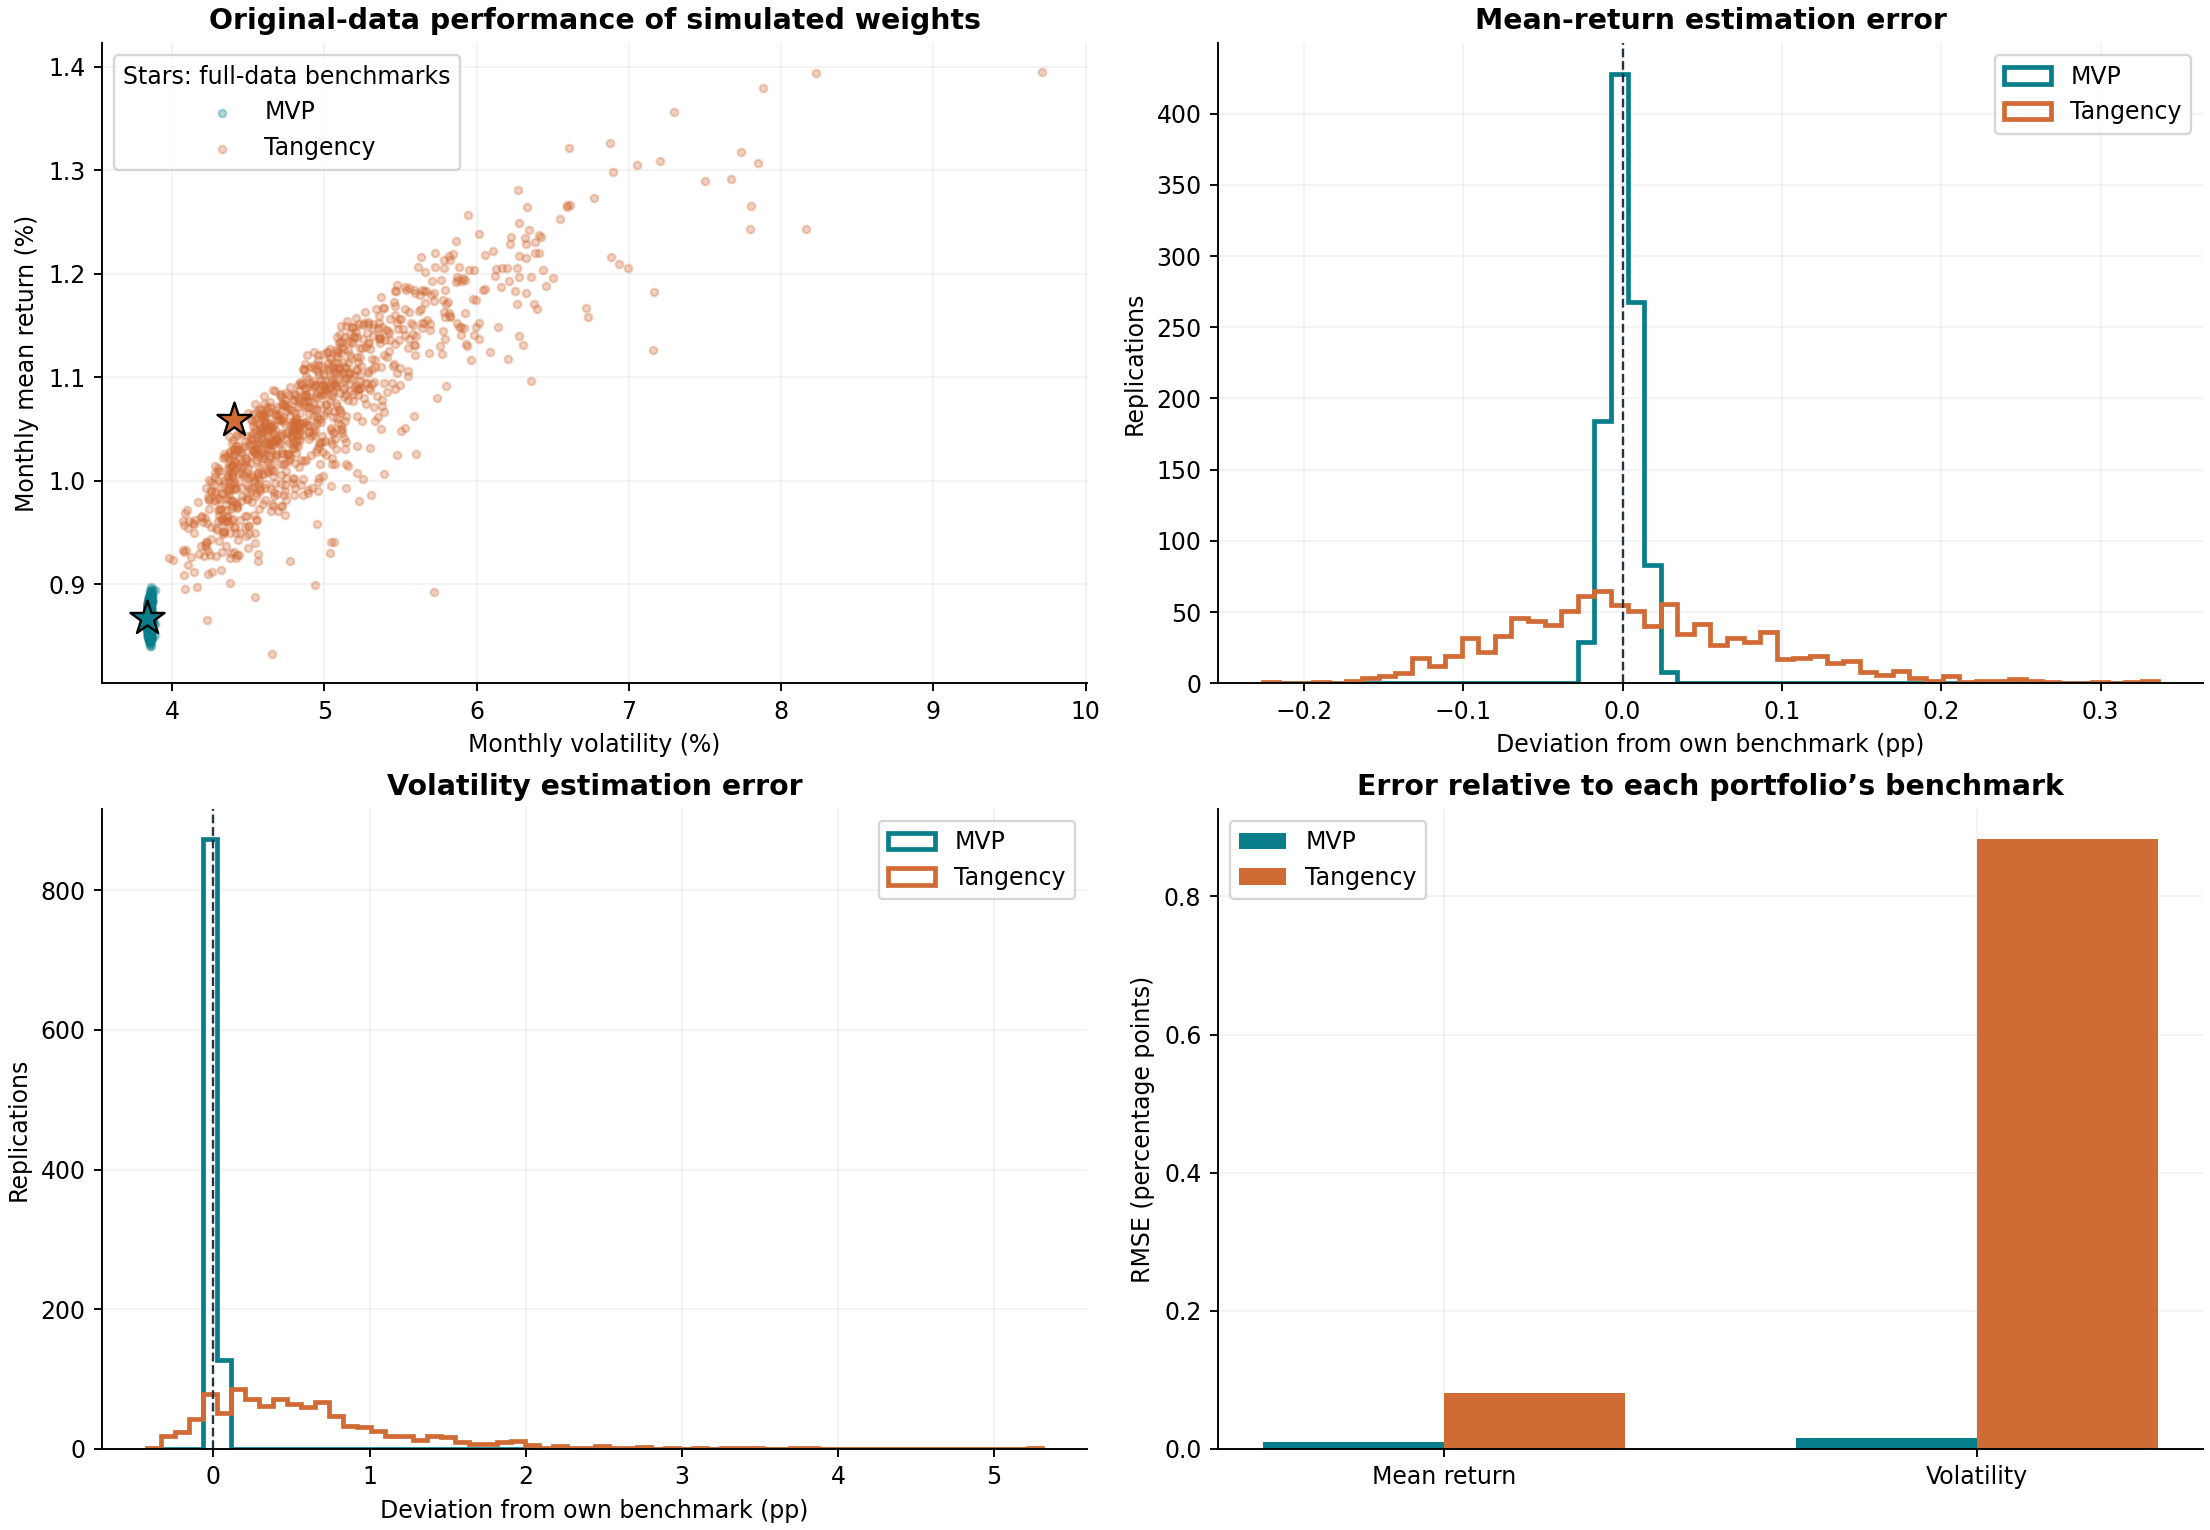
\includegraphics[width=\textwidth]{chatgpt_simulation_chart.png}
\caption{The chart produced by ChatGPT's script, reproduced from its own HTML
report. Stars mark the full-data benchmark portfolios.}
\label{fig:llm_chart}
\end{figure}

A small data analysis difference: it re-factorizes the covariance matrix on
every draw rather than reusing a single Cholesky factor, which is correct but
slower.

\item \textbf{Did the LLM correctly apply the simulated weights to the actual
returns?} Yes. Jorion's logic implies that no simulated portfolio should ever
beat the true optimum once judged against the original mean and covariance,
and none did for either portfolio in this test. If weights were evaluated on
the simulated sample, it would have failed this test constantly; the LLM got
the key distinction right here.

\item \textbf{Does the LLM correctly predict which portfolio has smaller
estimation error, and does its economic explanation hold up?}
\begin{itemize}
\item \textbf{Prediction.} Correct. ChatGPT's own generated report reproduces
the same asymmetry we found (Table~\ref{tab:llm_output}): the MVP has the
smaller estimation error in both mean and volatility, matching our own
Table~\ref{tab:q1de} and Figure~\ref{fig:q1d}.

\begin{table}[H]
\centering
\caption{Estimation-error metrics as reported in ChatGPT's own generated
output, \texttt{portfolio\_simulation\_report.html}.}
\small
\begin{tabular}{lrr}
\toprule
Metric & MVP & Tangency \\
\midrule
Mean-return RMSE (pp) & 0.0095 & 0.0817 \\
Volatility RMSE (pp) & 0.0160 & 0.8827 \\
Weight RMSE (pp of allocation) & 4.0318 & 28.2099 \\
\bottomrule
\end{tabular}
\label{tab:llm_output}
\end{table}

\item \textbf{Explanation.} Also correct. It attributes the gap to the MVP
depending only on the covariance matrix while the tangency portfolio
additionally depends on the noisy mean vector. It also separately notes that
MVP volatility sits at a variance minimum, so weight errors cost only a
second-order amount.
\end{itemize}

\end{itemize}

\subsection{Question 1(e): Empirical Row Bootstrap Simulation}

We repeat the experiment under the empirical distribution. Each simulation
draws $T = 1200$ month indices uniformly with replacement from
$\{1, \ldots, T\}$ and takes the corresponding rows of the actual return
matrix, so all ten industry returns for a sampled month stay together.
Sampling whole rows preserves the contemporaneous cross-sectional dependence
and the non-normal shape of the marginal distributions, while destroying
serial dependence such as volatility clustering. As before, weights are
estimated on the bootstrap sample and applied to the actual returns, 1{,}000
times. Results are in Table~\ref{tab:q1de} alongside the normal simulation.

\begin{figure}[H]
\centering

\includegraphics[width=\textwidth]{q1e_bootstrap_clouds.png}
\caption{Question 1(e). Weights estimated on empirical row-bootstrap samples
and applied to the actual industry returns, 1{,}000 simulations. Axes are
identical to Figure~\ref{fig:q1d} so the two experiments can be compared
directly.}
\label{fig:q1e}
\end{figure}

% Numbers available for this discussion:
%   - The answer is asymmetric, which is the interesting part:
%       MVP:      bootstrap dispersion is 1.83x the normal in realized mean
%                 and 2.14x in realized standard deviation.
%       Tangency: 1.01x and 1.00x, essentially unchanged.
%   - Interpretation: fat tails and skewness in actual monthly returns hurt the
%     covariance estimate that drives the MVP, so the MVP cloud widens.
%     Tangency error is already dominated by noise in mu-hat, so switching from
%     the normal to the empirical distribution adds nothing on top.
%   - The ordering is unchanged: the tangency cloud is still far wider than the
%     MVP cloud under the bootstrap (4.6x in mean, 45.0x in standard deviation).
%   - Limitation worth naming: the row bootstrap treats months as i.i.d., so it
%     ignores volatility clustering; a block bootstrap would relax this.
\paragraph{Discussion.}
\begin{itemize}
\setlength{\itemsep}{4pt}\setlength{\parskip}{0pt}

\item \textbf{The bootstrap raises estimation error for the MVP and leaves the
tangency portfolio unchanged.} Table~\ref{tab:q1de} shows the MVP spreading
roughly twice as wide under the bootstrap on both the realized mean and the
realized standard deviation, while the tangency figures are effectively
identical under the two samplers. We repeated the comparison across twenty
independent seed pairs and the split holds every time.

\item \textbf{Fat tails explain the split, because they affect the two inputs
differently.} Monthly industry returns are strongly non-normal: Jarque-Bera
rejects normality for all ten industries and average excess kurtosis is above
seven. The sampling variance of a mean depends only on the second moment, so
fat tails leave the mean vector exactly as precise as it was. The sampling
variance of a variance carries a term in excess kurtosis, which here roughly
doubles its standard error. The bootstrap therefore makes the covariance
matrix about twice as noisy and does nothing at all to the mean vector.

The MVP uses only the covariance matrix, so it absorbs that inflation in full,
and its extra dispersion comes out close to what the kurtosis predicts. For
the tangency portfolio we split the error into a part driven by the mean
vector and a part driven by the covariance matrix, and almost all of it comes
from the mean. The bootstrap inflates the smaller part, which barely moves the
total.

\item \textbf{The conclusion from part (d) survives.} The tangency cloud
remains far wider than the MVP cloud under the bootstrap, so switching to the
empirical distribution narrows the gap without coming close to closing it. One
caveat: the row bootstrap samples months independently, so it reproduces fat
tails and contemporaneous correlation while destroying volatility clustering.
It captures one way the normal assumption fails and misses another.

\end{itemize}

% =====================================================================
% Question 2 (three-asset hand calculation) and Question 3 (robust
% portfolio construction) are written by the other group members.  Paste
% them in below as \section{...} blocks before \end{document}.
% =====================================================================

\end{document}
